\documentclass{article}
\usepackage{tikz}
\usetikzlibrary{decorations.pathmorphing}

\begin{document}

\begin{figure}
\centering
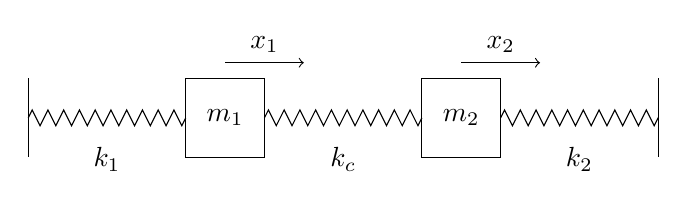
\begin{tikzpicture}
  \draw (0,1)--(0,-0);
  \draw (8,1)--(8,-0);

  % Left spring
  \draw [decorate,decoration={zigzag,segment length=2mm,amplitude=1mm}] (0,0.5) -- (2,0.5);
  \node [above] at (1,-0.3) {$k_1$};

  % Left mass m1
  \draw (2,0) rectangle node {$m_1$} (3,1);
  \draw[->] (2.5,1.2) -- node[above]{$x_1$} (3.5,1.2);

  % Middle spring
  \draw [decorate,decoration={zigzag,segment length=2mm,amplitude=1mm}] (3,0.5) -- (5,0.5);
  \node [above] at (4,-0.3) {$k_c$};

  % Right mass m2
  \draw (5,0) rectangle node {$m_2$} (6,1);
  \draw[->] (5.5,1.2) -- node[above]{$x_2$} (6.5,1.2);

  % Right spring
  \draw [decorate,decoration={zigzag,segment length=2mm,amplitude=1mm}] (6,0.5) -- (8,0.5);
  \node [above] at (7,-0.3) {$k_2$};
\end{tikzpicture}
\end{figure}

\end{document}

